\subsection{Messung der longitudinalen Relaxationszeit}
Bei allen folgenden Messungen wurde der Untergrund vor dem ersten Puls (etwa 50 Werte) analysiert. Alle Werte wurden um den Mittelwert korrigiert. Für den Fehler der einzelnen Werte wurde der RMS-Wert des Untergrundes verwendet.
\subsubsection{Sättigungszurückgewinnung}
\begin{figure}[h]
  \begin{subfigure}[h]{0.5\textwidth}
    \centering
    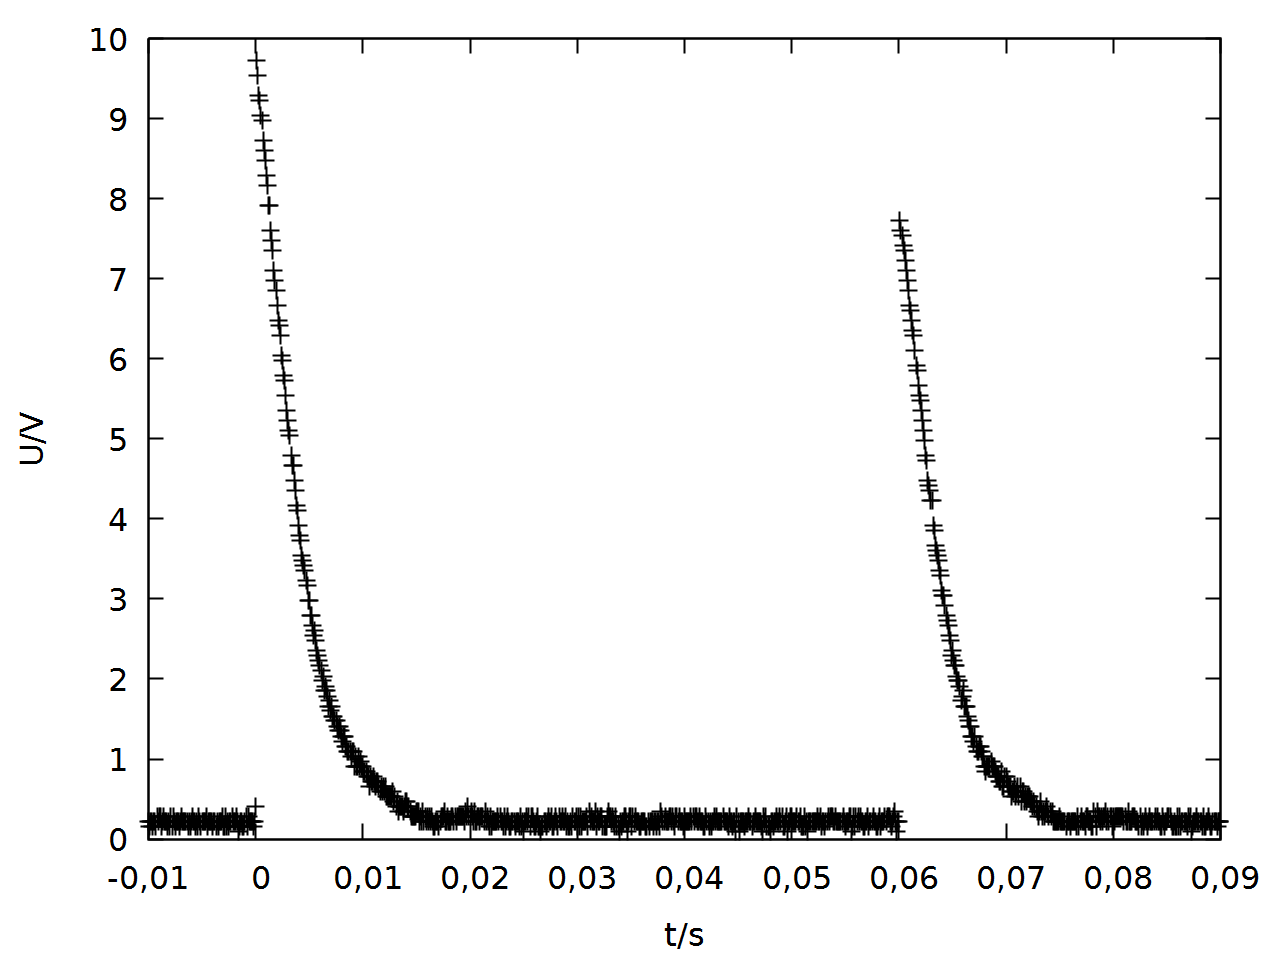
\includegraphics[width=\linewidth]{data/p402_443_data/saettigungszurueckgewinnung/plot_81.png}
    \subcaption{Ausgabe für $\tau=60\si{\milli\second}$}
    \label{fig:sat_bsp}
  \end{subfigure}%
  \begin{subfigure}[h]{0.5\textwidth}
    \centering
    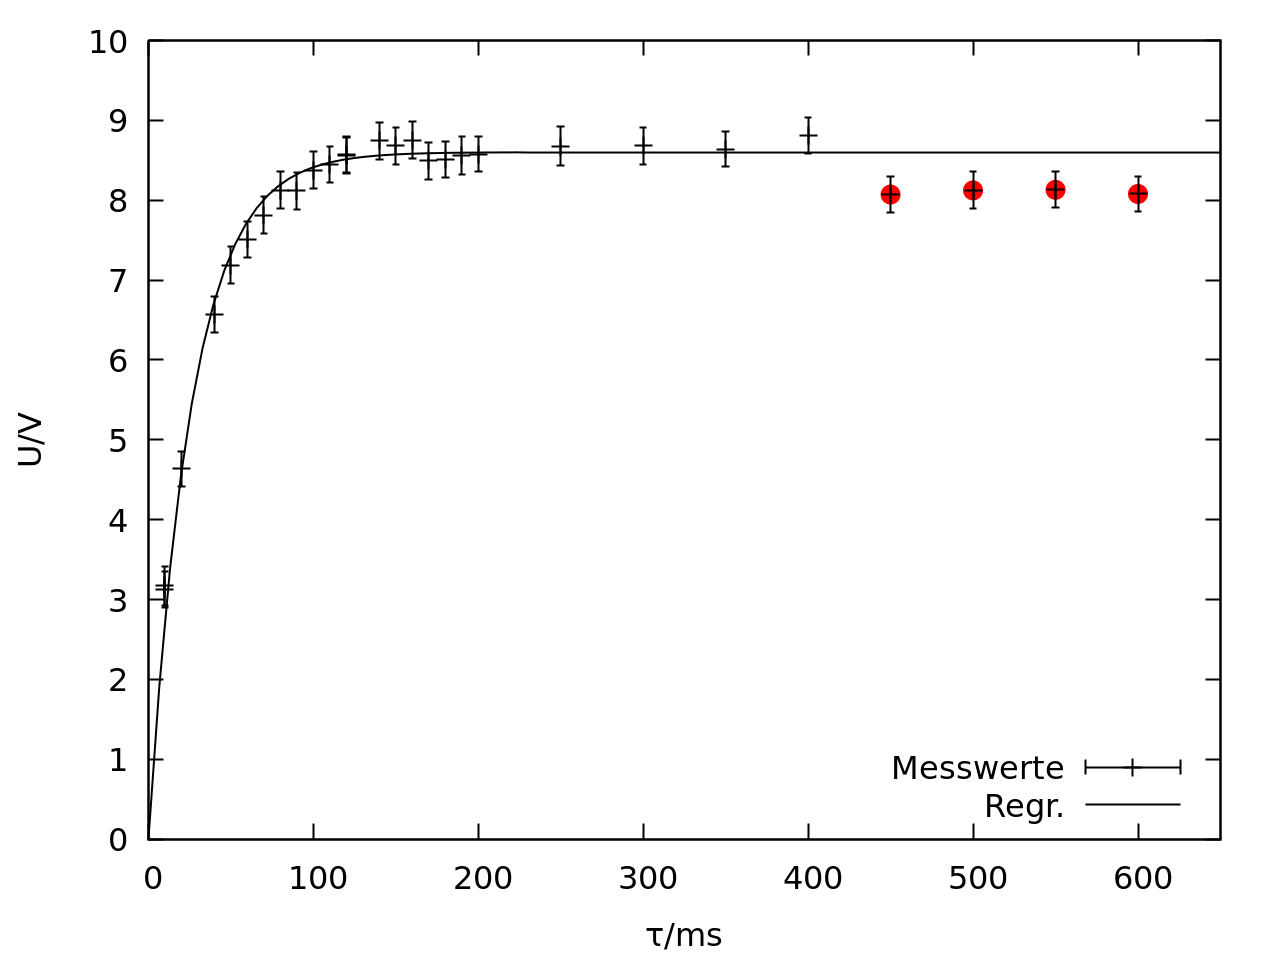
\includegraphics[width=\linewidth]{data/p402_443_data/saettigungszurueckgewinnung/out_sat.png}
    \subcaption{Anpassung an die bestimmten Amplituden (rot: nicht für die Anpassung verwendet)}
    \label{fig:sat_data}
  \end{subfigure}
  \caption{Sättigungszurückgewinnung}
\end{figure}

Aus den Daten des Oszilloskops (siehe Abb. \ref{fig:sat_bsp}) wird das zweite Maximum bestimmt und über der Wartezeit $\tau$ aufgetragen (siehe Abb. \ref{fig:sat_data}). Während der Auswertung fiel uns auf, dass manchmal die erwartete Wartezeit $\tau$ zwischen den Pulsen nicht der im Plot erkennbaren entsprach. Vermutlich haben wir da die falsche Zeit eingestellt. Bei diesen Werten wurde die Wartezeit dann auf den Wert aus dem Plot gesetzt. Deswegen sind die Datenpunkte nicht immer äquidistant. 

An die Daten wird die Funktion $$U(\tau) = U_0\left(1-\exp{\left(-\frac{\tau}{T_1}\right)}\right)$$ angepasst, die resultierenden Parameter sind $U_0 = (8,60\pm 0,05)\si{\volt}$ und $T_1 = (26,2\pm 0,8) \si{\milli\second}$. Für die Regression haben wir die rot eingefärbten Punkte vernachlässigt. Diese wurden in einer anderen Einstellung des Messbereiches aufgenommen und liegen deutlich unterhalb der Punkte davor. Wir schätzen, dass die Einstellung am Oszilloskop die Werte verändert hat.

\subsection{Polarisationszurückgewinnung}
\begin{figure}[h]
  \begin{subfigure}[h]{0.5\textwidth}
    \centering
    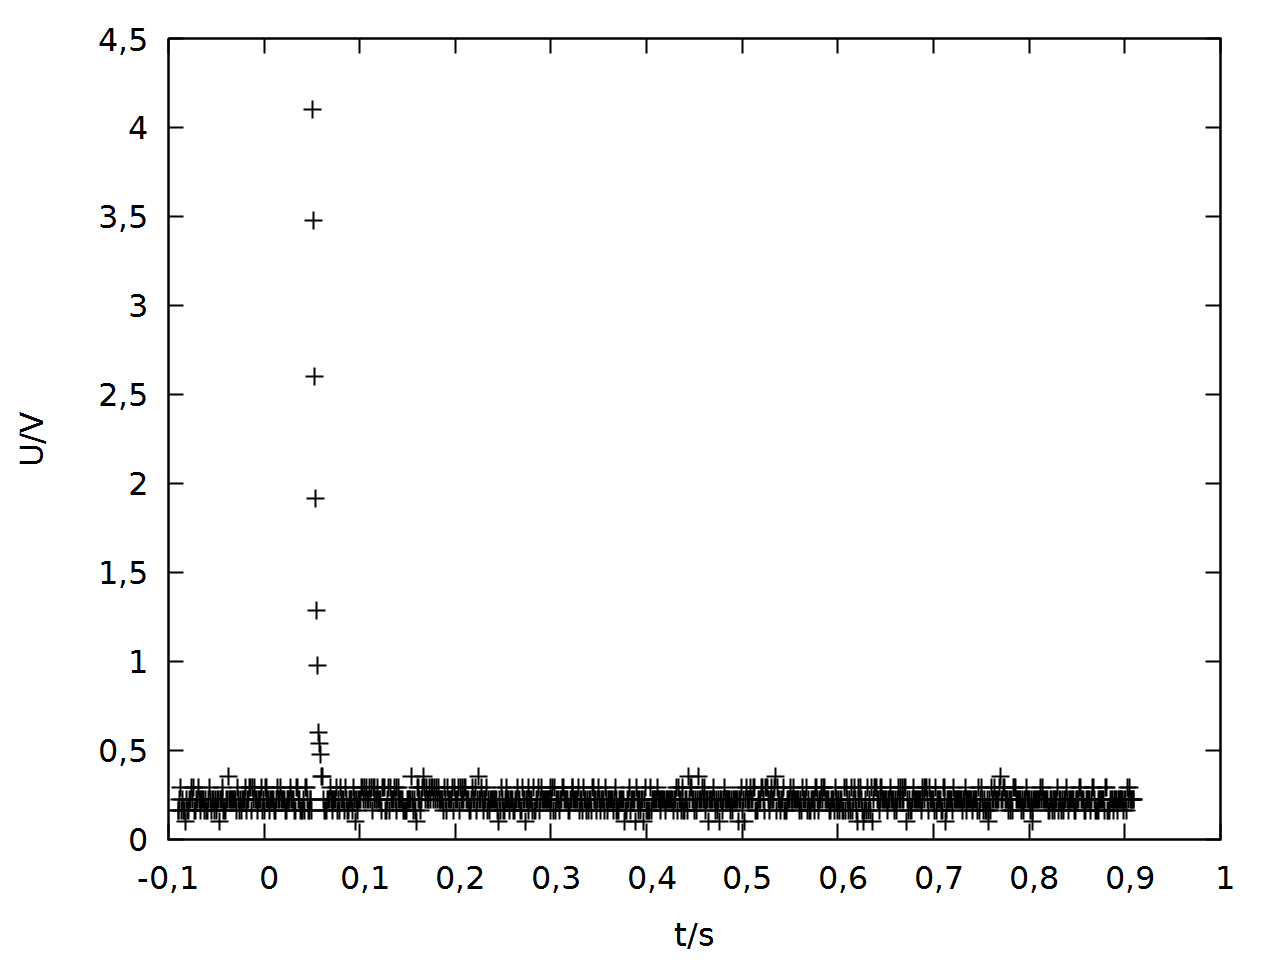
\includegraphics[width=\linewidth]{data/p402_443_data/polarisationszurueckgewinnung/plot_110.png}
    \subcaption{Ausgabe für $\tau=50\si{\milli\second}$}
    \label{fig:pol_bsp}
  \end{subfigure}%
  \begin{subfigure}[h]{0.5\textwidth}
    \centering
    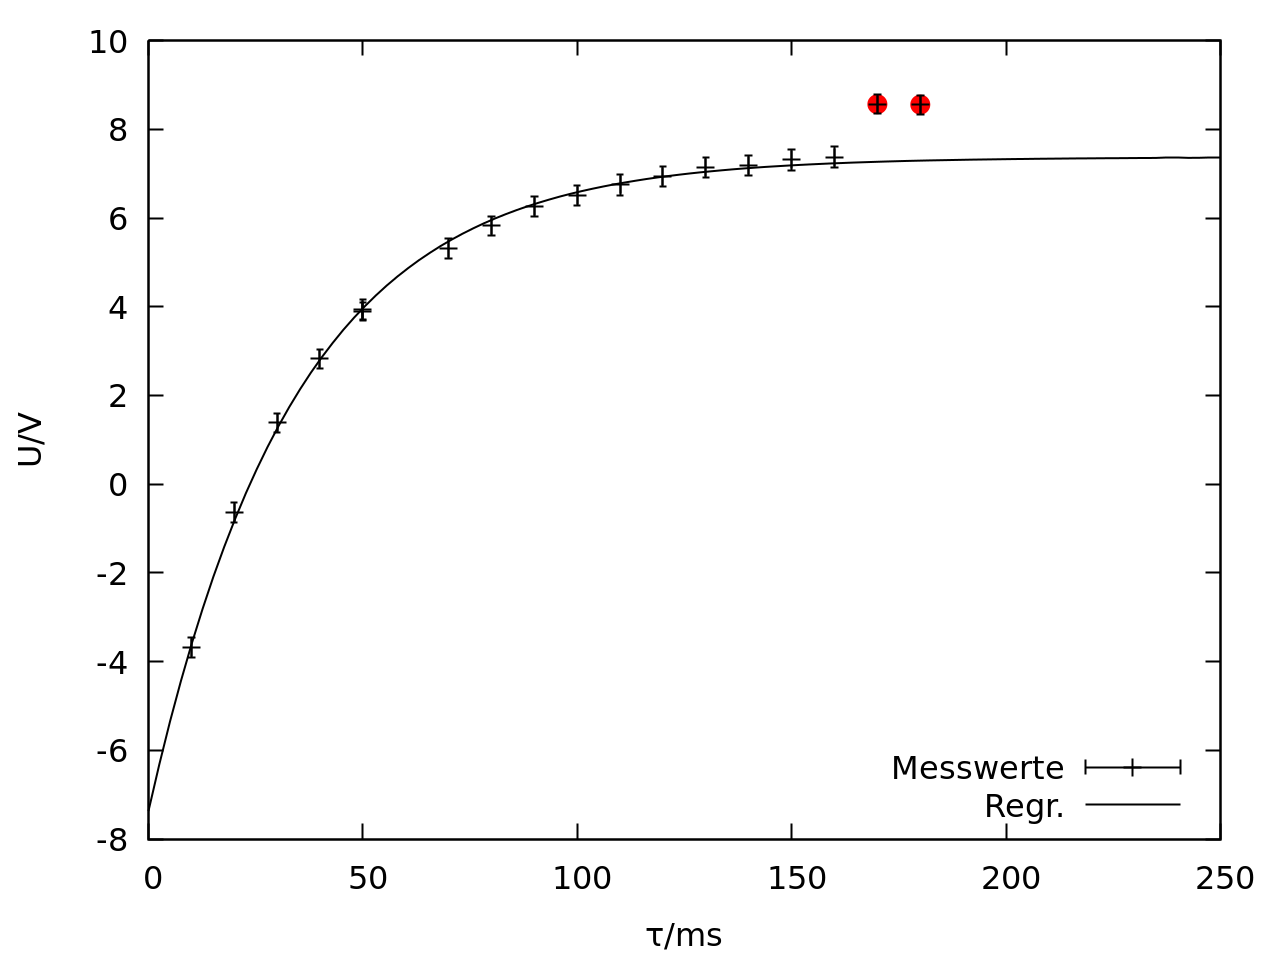
\includegraphics[width=\linewidth]{data/p402_443_data/polarisationszurueckgewinnung/out_pol.png}
    \subcaption{Anpassung an die bestimmten Amplituden (rot: nicht für die Anpassung verwendet)}
    \label{fig:pol_data}
  \end{subfigure}
  \caption{Polarisationszurückgewinnung}
\end{figure}
In diesem Versuchsteil stürzte das Oszilloskop während einer Messung ab. Auf den danach aufgenommen Datensätzen ist nur Hintergrundrauschen zu erkennen, wodurch wir sie nicht zur Auswertung verwenden konnten. Wir denken, dass es sich dabei um einen Softwarefehler des Oszilloskops handelt.\\

Da die Polarisation zu Beginn in negative $z$-Richtung zeigt werden die ersten zwei Spannungswerte mit $-1$ multipliziert.  
Aus den Daten des Oszilloskops (siehe Abb. \ref{fig:pol_bsp}) wird das Maximum bestimmt und über der Wartezeit $\tau$ aufgetragen (siehe Abb. \ref{fig:pol_data}). Man kann erkennen, dass es nur wenige Datenpunkte im Bereich des Maximums gibt und man somit die wirkliche Amplitude des Signales nicht sehr genau bestimmen kann. Da wir diesen Fehler nicht abschätzen können, haben wir beschlossen wieder den Fehler des Hintergrundes zu verwenden. In Abb. \ref{fig:pol_data} liegt die angepasste Funktion aber im Fehlerbereich aller Messwerte.

Die Anpassung $$U(\tau) = U_0\left(1-2\exp{\left(-\frac{\tau}{T_1}\right)}\right)$$ ergibt $U_0 = (7,4\pm 0,1)\si{\volt}$ und $T_1 = (34,8\pm 0,8) \si{\milli\second}$. Die rot eingefärbten Daten wurden wieder mit einer anderen Messbereichseinstellung aufgenommen und aufgrund ihrer starken Abweichung nicht für die Anpassung verwendet.\\

Die beiden Ergebnisse für die longitudinale Relaxationszeit $(26,2\pm 0,8) \si{\milli\second}$ und $(34,8\pm 0,8) \si{\milli\second}$ liegen zwar in der gleichen Größenordnung, weichen aber dennoch außerhalb der Fehlertoleranz voneinander ab. Wie man bei den Daten aber schon sehen konnte, gab es durchaus Unterschiede bei den gemessenen Spannungen, je nachdem welche Auflösung am Oszilloskop eingestellt war. Diese betrug bei der Sättigungszurückgewinnungsmethode 20\si{\milli\second}/div und bei der Polarisationszurückgewinnungsmethode 100\si{\milli\second}/div. Somit könnten durchaus andere Spannungen gemessen worden sein.\\
Eine mögliche weitere Fehlerquelle für die Polarisationszugrückgewinnung könnte der unbekannte Fehler auf die Amplitude des Signals aufgrund weniger Daten im Bereich des Peaks sein.
%In Abb. \ref{fig:pol_error} wurde ein Fit an den Daten der Polarisationsrückgewinnung mit festgelegter Relaxationszeit $T_1 = 26,2 \si{\milli\second}$ durchgeführt. Man erkennt, dass für etwa doppelte Fehler dies ein realistischer Fit wäre. Allerdings ist dann auch die Sättigungsspannung mit $U_0 = (6,7\pm 0,2)\si{\volt}$ deutlich kleiner als die bei der Sättigungsrückgewinnungsmethode ($U_0 = (8,60\pm 0,05)\si{\volt}$). 

%\begin{figure}[h]
%\centering
%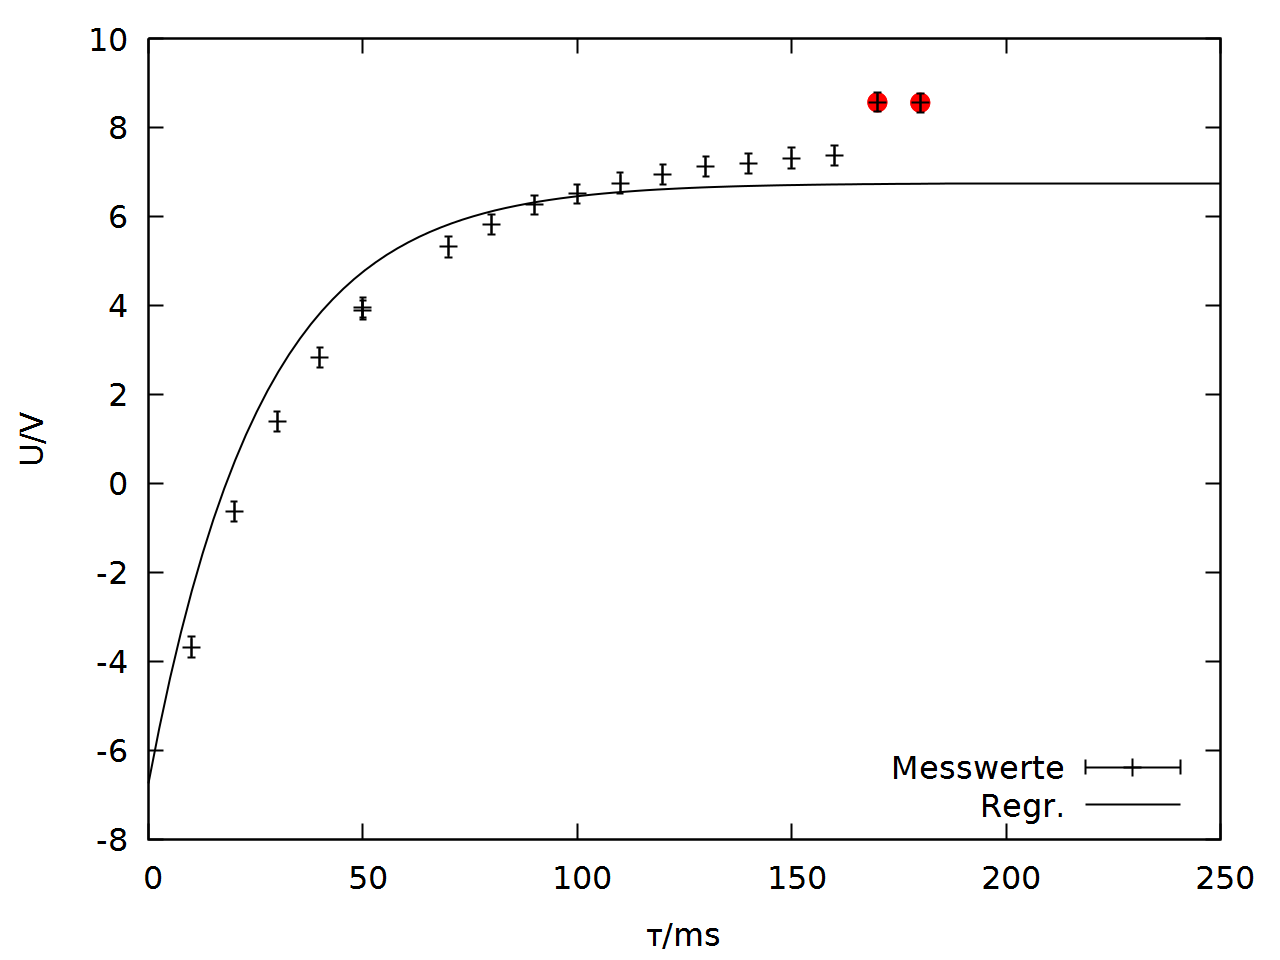
\includegraphics[width=0.75\linewidth]{data/p402_443_data/polarisationszurueckgewinnung/out_pol_2.png}
%\caption{(Polarisationszurückgewinnung) Fit mit $T_1 = 26,2 \si{\milli\second}$}
%\label{fig:pol_error}
%\end{figure}

\subsection{Messung der transversalen Relaxationszeit}
\subsubsection{Effektive transversale Relaxationszeit}
Um die effektive transversale Relaxationszeit zu bestimmen, wird an das FID-Signal ein exponentieller Abfall $$U(\tau) = U_0\exp{\left(-\frac{\tau}{T_2^*}\right)}$$ angepasst (siehe Abb. \ref{fig:hahn_fid}).

\begin{figure}[h]
\centering
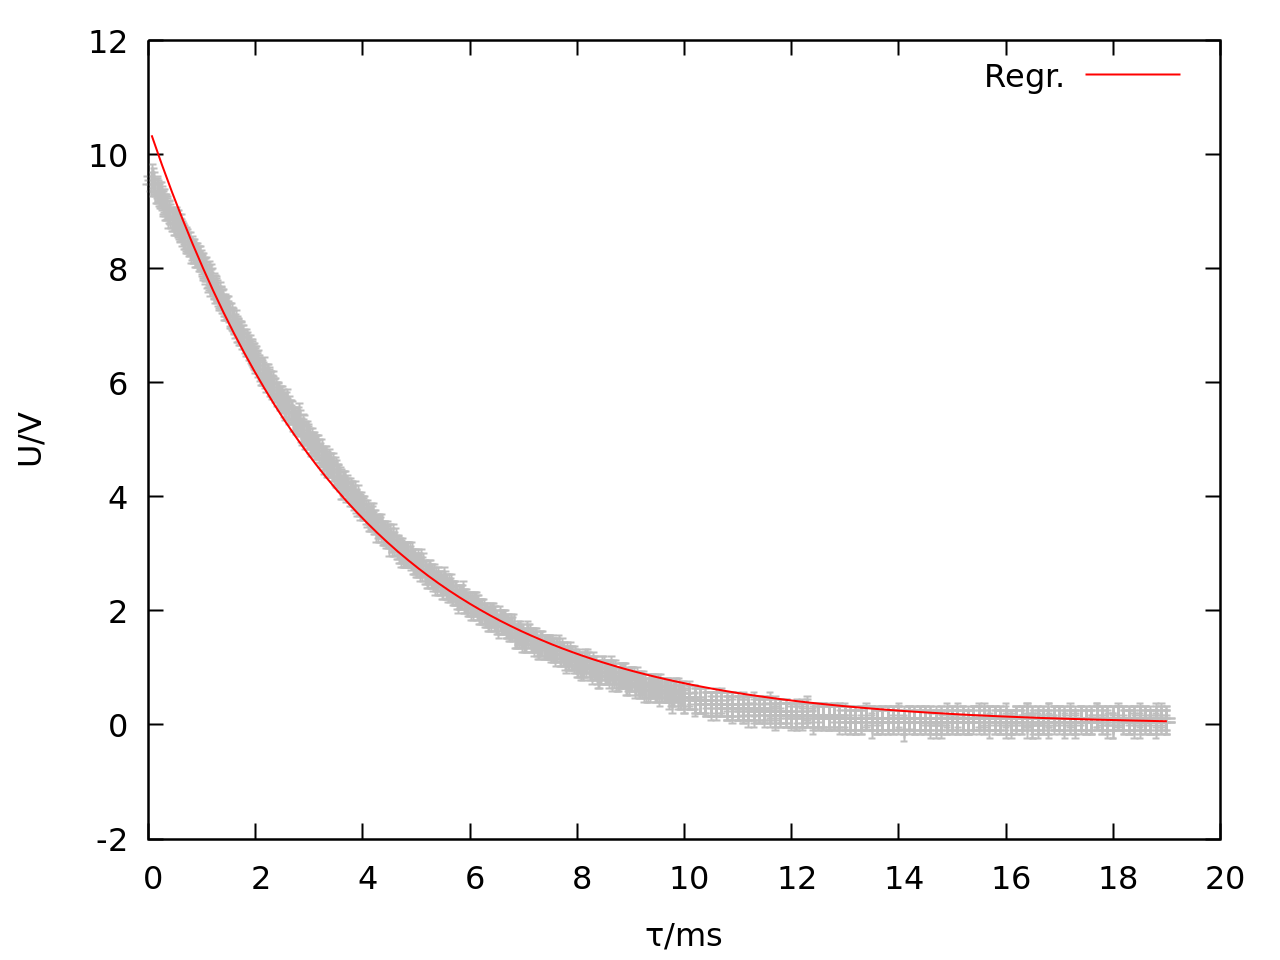
\includegraphics[width=0.75\linewidth]{data/p402_443_data/hahn_sequenz/out_fid.png}
\caption{FID mit Anpassung exponentiellen Zerfalls}
\label{fig:hahn_fid}
\end{figure}

Die Parameter sind $U_0 = (10,51\pm 0,03)\si{\volt}$ und $T_2^* = (3,75355\pm 0,02) \si{\milli\second}$. 

\subsubsection{Hahn-Spinecho}
Aus den Daten des Oszilloskops (siehe Abb. \ref{fig:hahn_bsp}) wird das zweite Maximum bestimmt und über der doppelten Wartezeit $2\tau$ aufgetragen (siehe Abb. \ref{fig:hahn_data}).

Daran wird nun eine exponentielle Funktion angepasst: $$U(\tau) = U_0\exp{\left(-\frac{2\tau}{T_2}\right)}$$. Die Anpassung ergibt $U_0 = (8,9\pm 0,1)\si{\volt}$ und $T_2 = (20,2\pm 0,6) \si{\milli\second}$.

\begin{figure}[h]
  \begin{subfigure}[h]{0.5\textwidth}
    \centering
    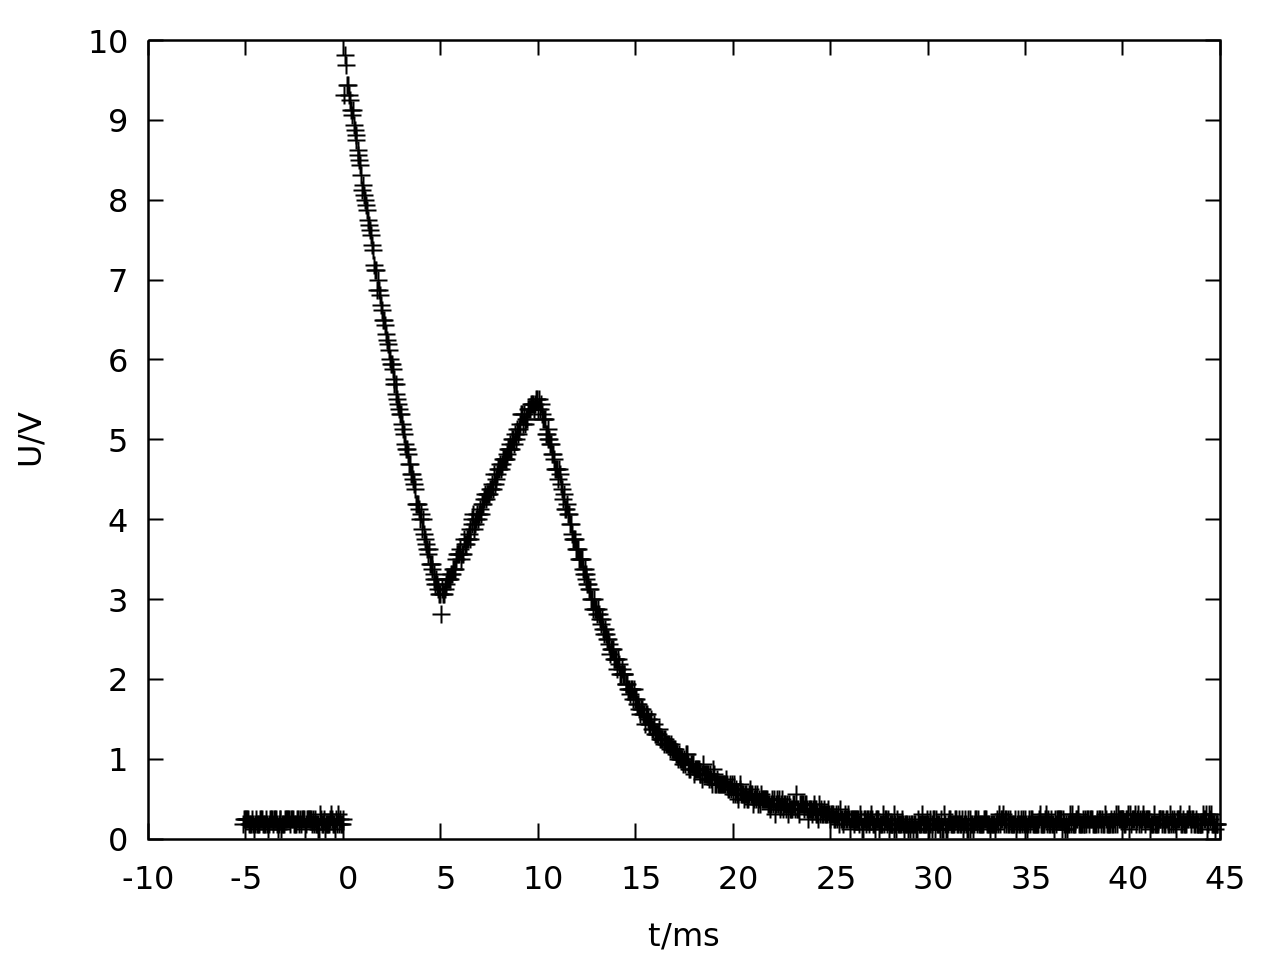
\includegraphics[width=\linewidth]{data/p402_443_data/hahn_sequenz/plot_146.png}
    \subcaption{Ausgabe für $\tau=50\si{\milli\second}$}
    \label{fig:hahn_bsp}
  \end{subfigure}%
  \begin{subfigure}[h]{0.5\textwidth}
    \centering
    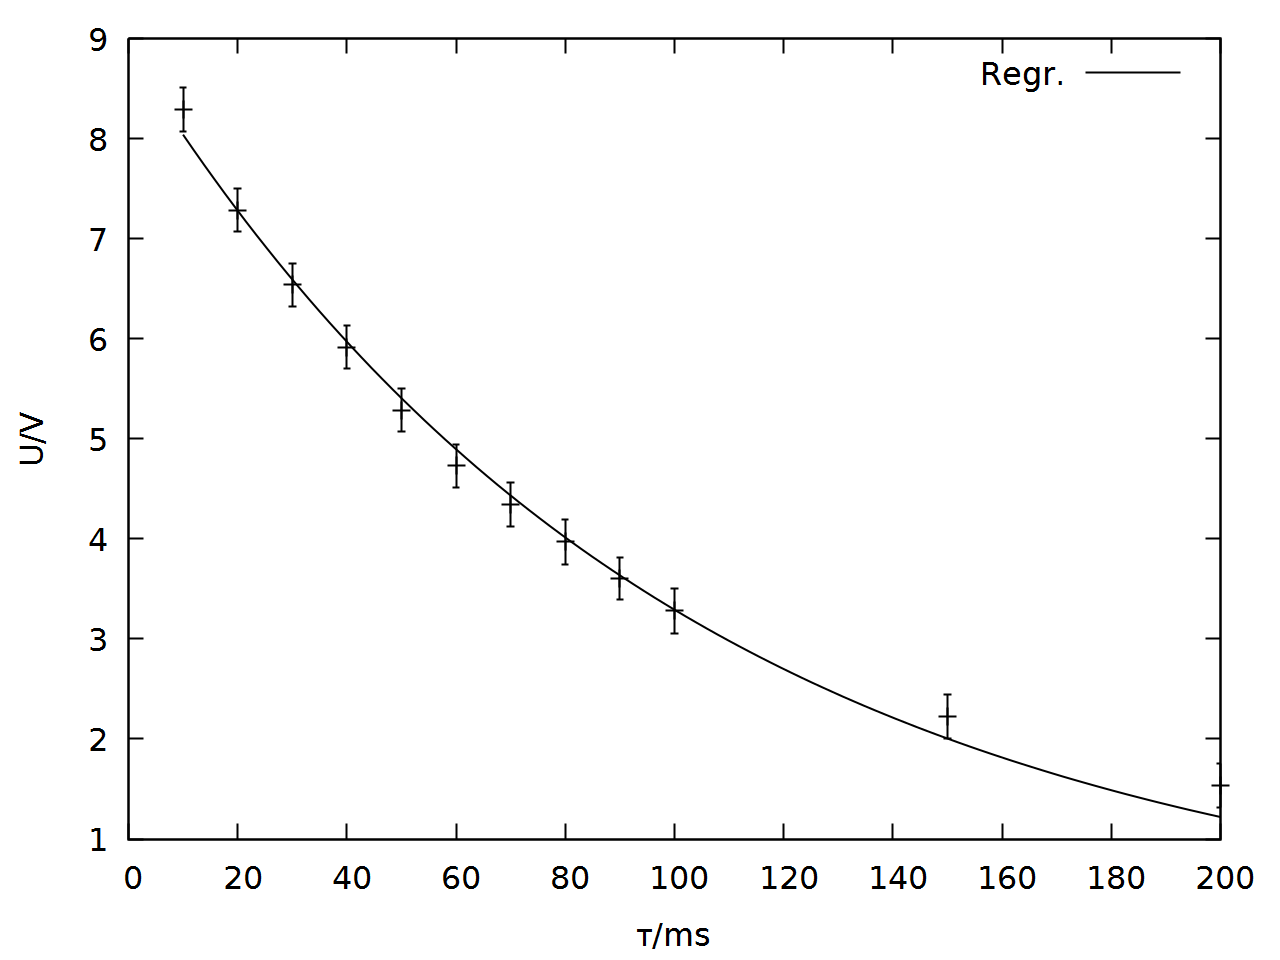
\includegraphics[width=\linewidth]{data/p402_443_data/hahn_sequenz/out_hahn.png}
    \subcaption{Anpassung an die bestimmten Amplituden}
    \label{fig:hahn_data}
  \end{subfigure}
  \caption{Hahn-Spinecho-Sequenz}
\end{figure}

\subsubsection{Carr-Purcell-Sequenz}
Aus den Daten des Oszilloskops (siehe Abb. \ref{fig:carr_raw}) werden die Positionen der lokalen Maxima bestimmt und über der Zeit $t$ aufgetragen (siehe Abb. \ref{fig:carr}).

Daran wird nun die exponentielle Funktion $$U(\tau) = U_0\exp{\left(-\frac{\tau}{T_2}\right)}$$ angepasst. Die Regression ergibt $U_0 = (8,9\pm 0,1)\si{\volt}$ und $T_2 = (19,2\pm 0,3) \si{\milli\second}$.\\

\begin{figure}[h]
  \begin{subfigure}[h]{0.5\textwidth}
    \centering
    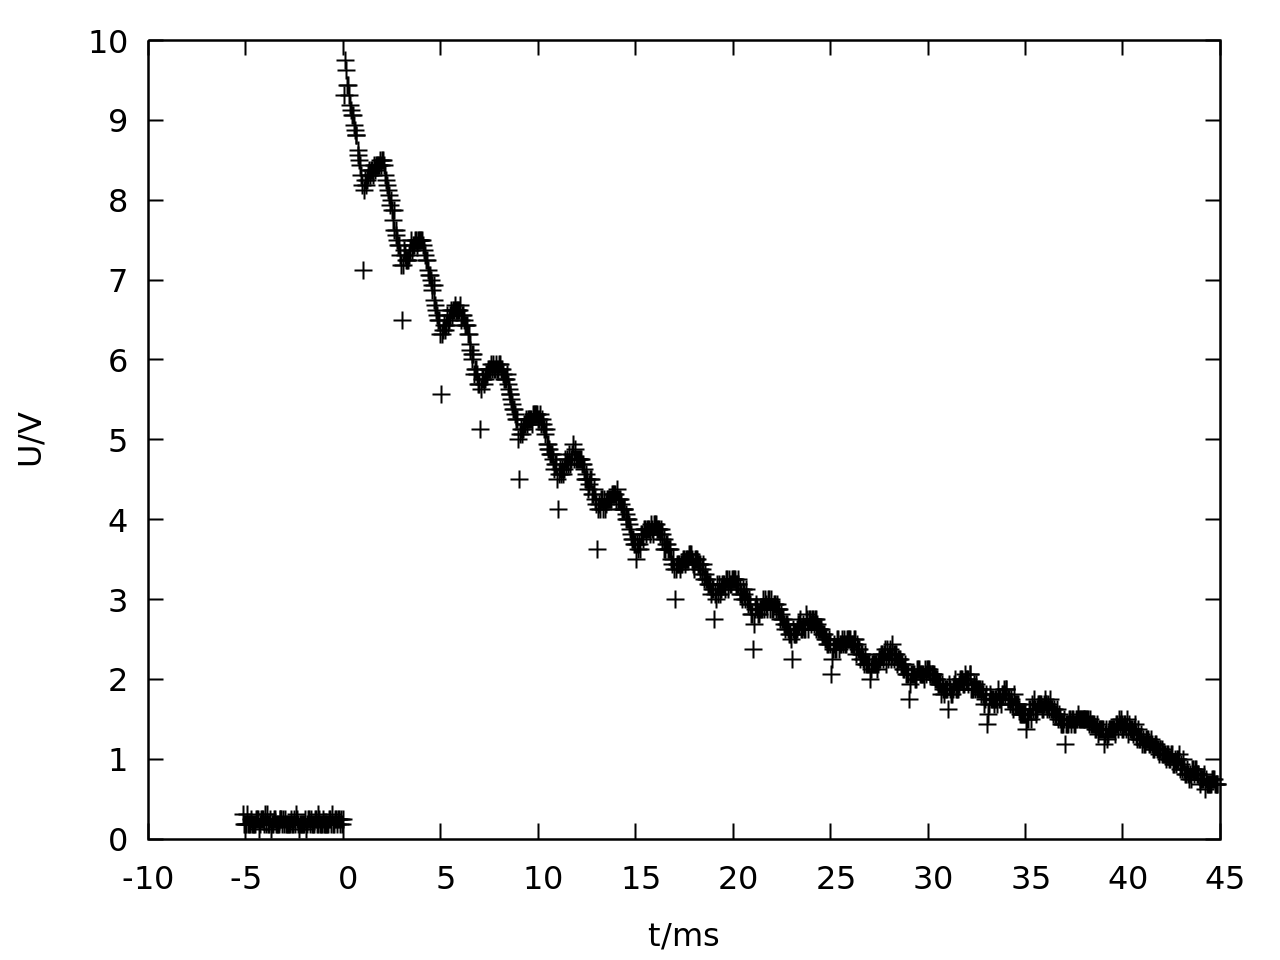
\includegraphics[width=\linewidth]{data/p402_443_data/carr_purcell_sequenz/plot_156.png}
    \subcaption{Ausgabe des Oszilloskops}
    \label{fig:carr_raw}
  \end{subfigure}%
  \begin{subfigure}[h]{0.5\textwidth}
    \centering
    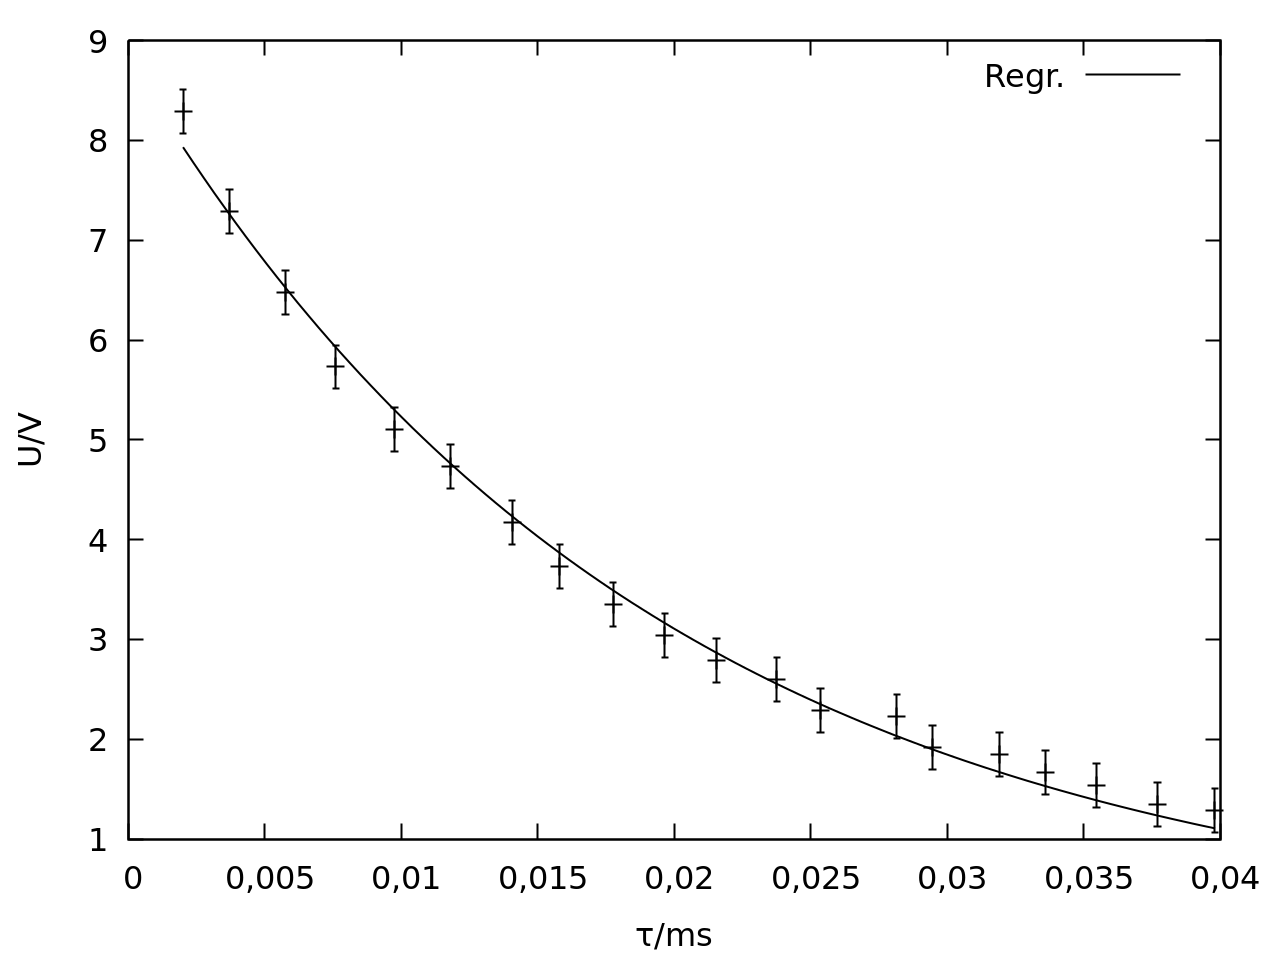
\includegraphics[width=\linewidth]{data/p402_443_data/carr_purcell_sequenz/out_carr.png}
    \subcaption{Anpassung an die bestimmten Amplituden}
    \label{fig:carr}
  \end{subfigure}
  \caption{Carr-Purcell-Sequenz}
\end{figure}

Ändert man die Pulslänge, so wandern die Maxima weiter auseinander. Für Abb. \ref{fig:carr_b} wurden die Magnetfeldgradienten verändert. Man kann erkennen, dass die Sequenz von einer anderen periodischen Funktion überlagert wird. Dies liegt daran, dass die Länge eines $\pi$-Pulses vom Magnetfeld abhängt. Das bedeutet, dass manche Protonenspins nicht genau um $180^\circ$ um die x-Achse gedreht werden und somit eine z-Komponente erhalten. Diese z-Komponente wird aufgrund des gleichen Drehsinns zunehmend größer (und nimmt später wieder ab, nachdem der Spin vollständig in z-Richtung polarisiert war). Dadurch nehmen die gemessenen x-y-Komponenten ab und das Signal verschwindet schneller.
 
\begin{figure}[h]
\centering
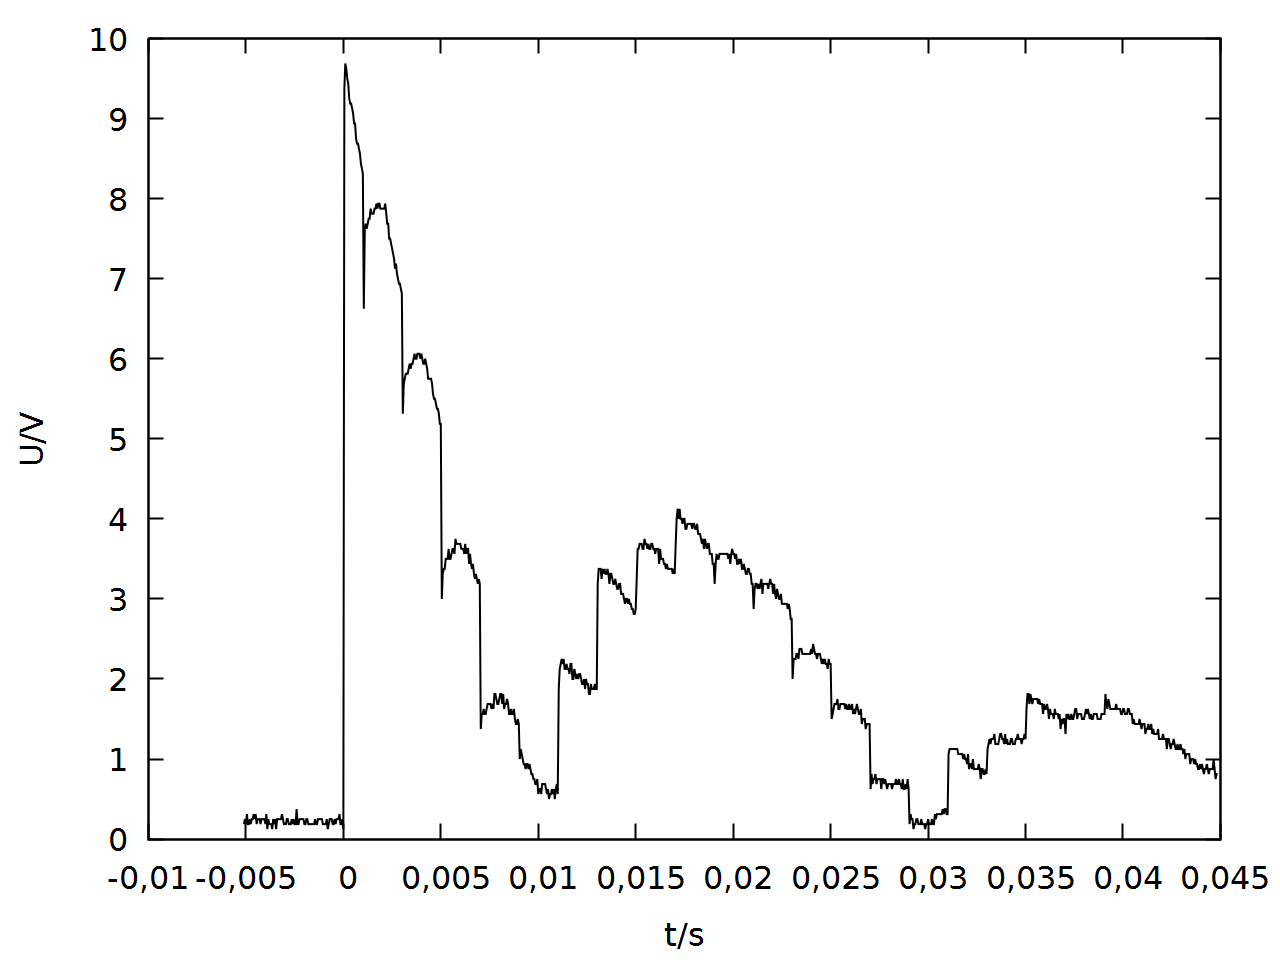
\includegraphics[width=0.75\linewidth]{data/p402_443_data/carr_purcell_sequenz/plot_157.png}
\caption{(Carr-Purcell-Sequenz) Nach Änderung der Magnetfeldgradienten}
\label{fig:carr_b}
\end{figure}
\newpage

\subsubsection{Meiboom-Gill-Sequenz}

\begin{figure}[h]
  \begin{subfigure}[h]{0.5\textwidth}
    \centering
    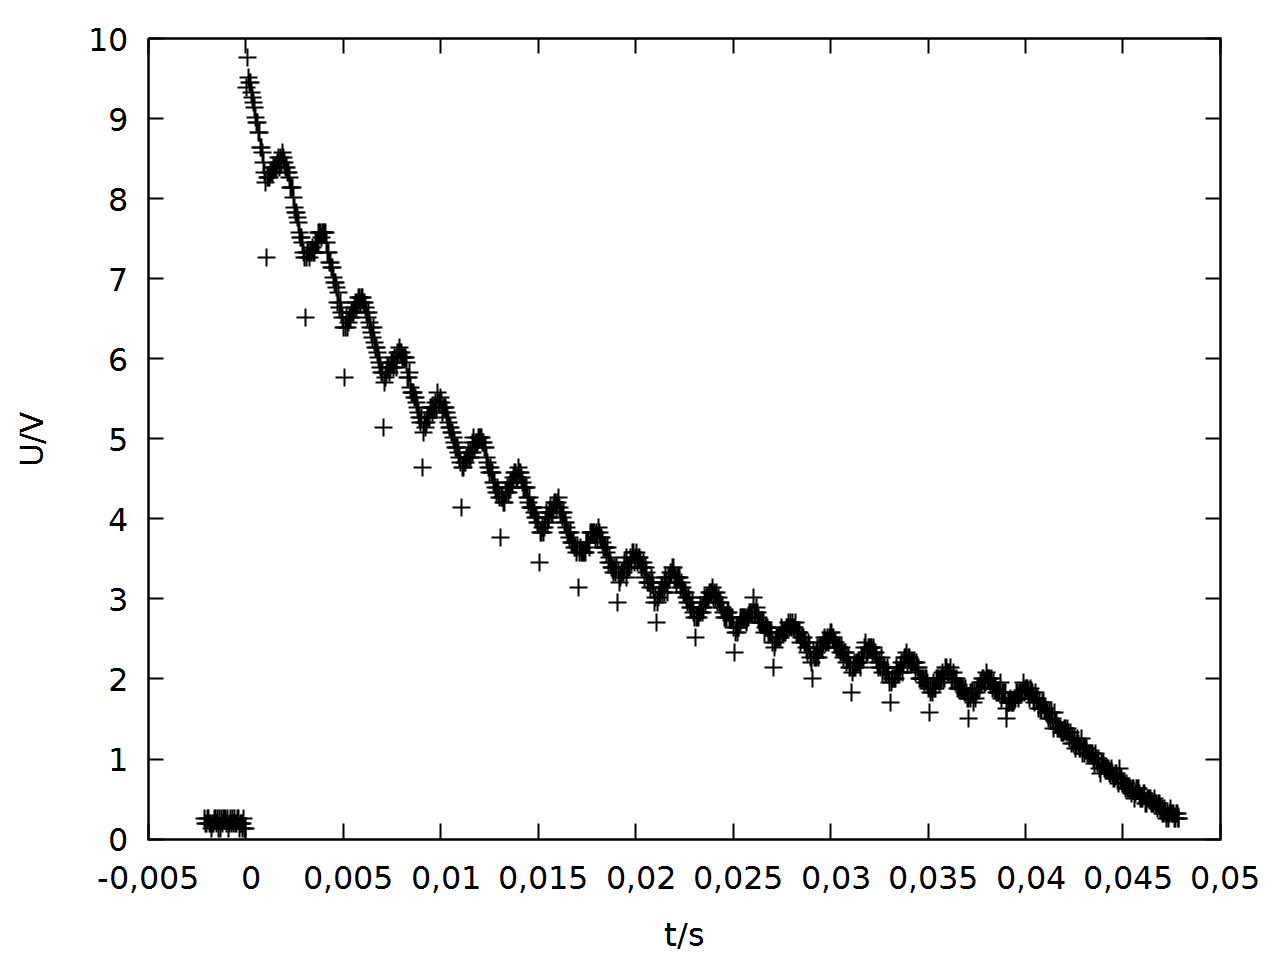
\includegraphics[width=\linewidth]{data/p402_443_data/meiboom_gill_sequenz/plot_159.png}
    \subcaption{Ausgabe des Oszilloskops}
    \label{fig:gill_raw}
  \end{subfigure}%
  \begin{subfigure}[h]{0.5\textwidth}
    \centering
    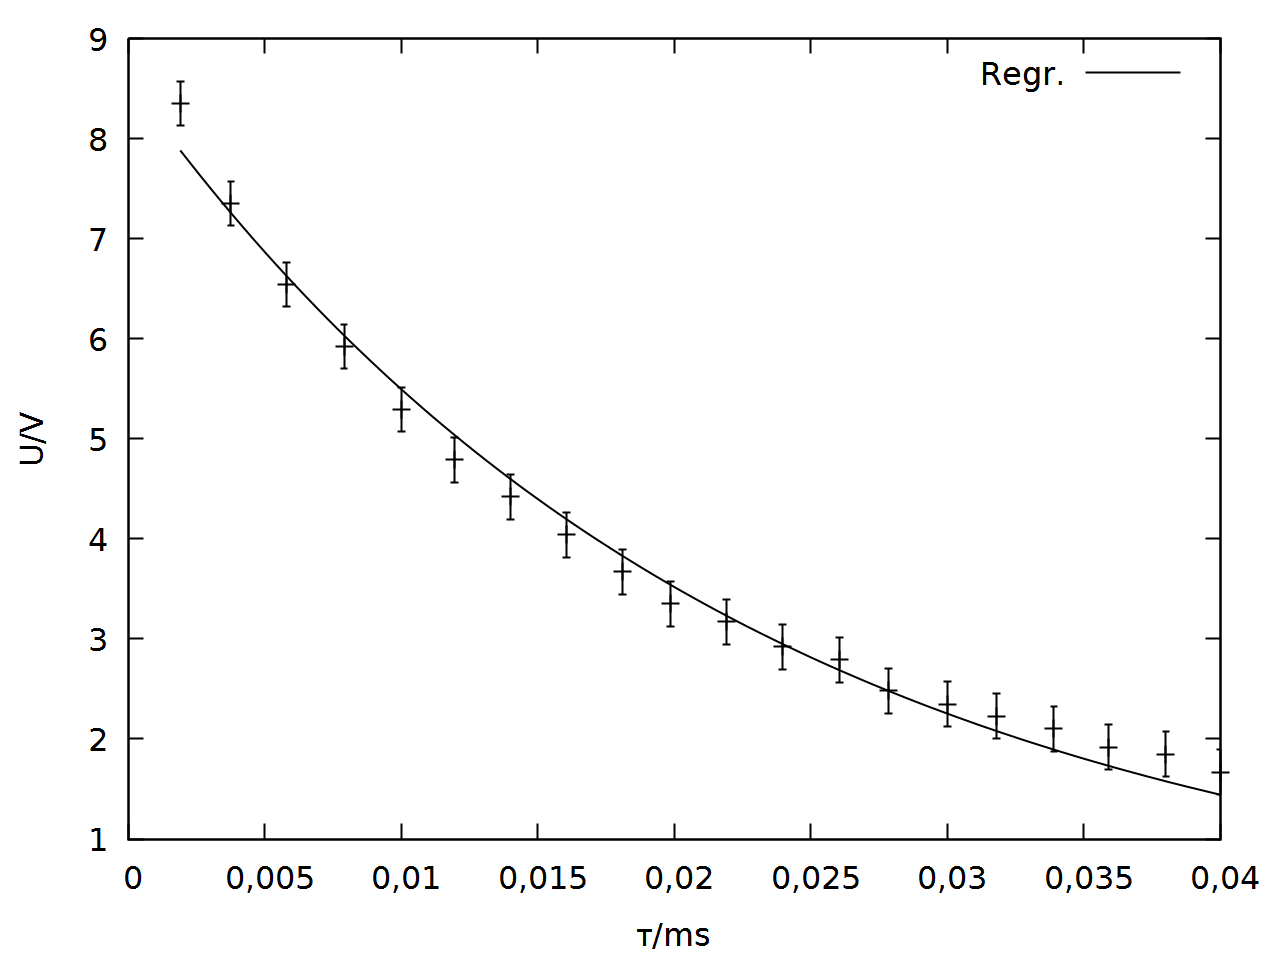
\includegraphics[width=\linewidth]{data/p402_443_data/meiboom_gill_sequenz/out_gill.png}
    \subcaption{Anpassung an die bestimmten Amplituden}
    \label{fig:gill}
  \end{subfigure}
  \caption{Meiboom-Gill-Sequenz}
\end{figure}
Die Auswertung von Abb. \ref{fig:gill_raw} erfolgt analog zur Carr-Purcell-Sequenz (siehe Abb. \ref{fig:gill}).

Die Regression $$U(\tau) = U_0\exp{\left(-\frac{\tau}{T_2}\right)}$$ ergibt $U_0 = (8,6\pm 0,1)\si{\volt}$ und $T_2 = (22,4\pm 0,6) \si{\milli\second}$.\\

Ändert man bei der Meiboom-Gill-Sequenz die Magnetfeldgradienten (siehe Abb. \ref{fig:gill_b}), fällt das Signal zwischen den Pulsen zwar schneller ab, die Lage der Maxima bleibt aber gleich. Durch den umgekehrten Drehsinn bei jedem zweitem Winkel dreht sich ein möglicherweise falscher $\pi$-Puls wieder um genau den gleichen Winkel zurück. Somit liegen alle Spins dann wieder in der x-y-Ebene.\\
  
\begin{figure}[h]
\centering
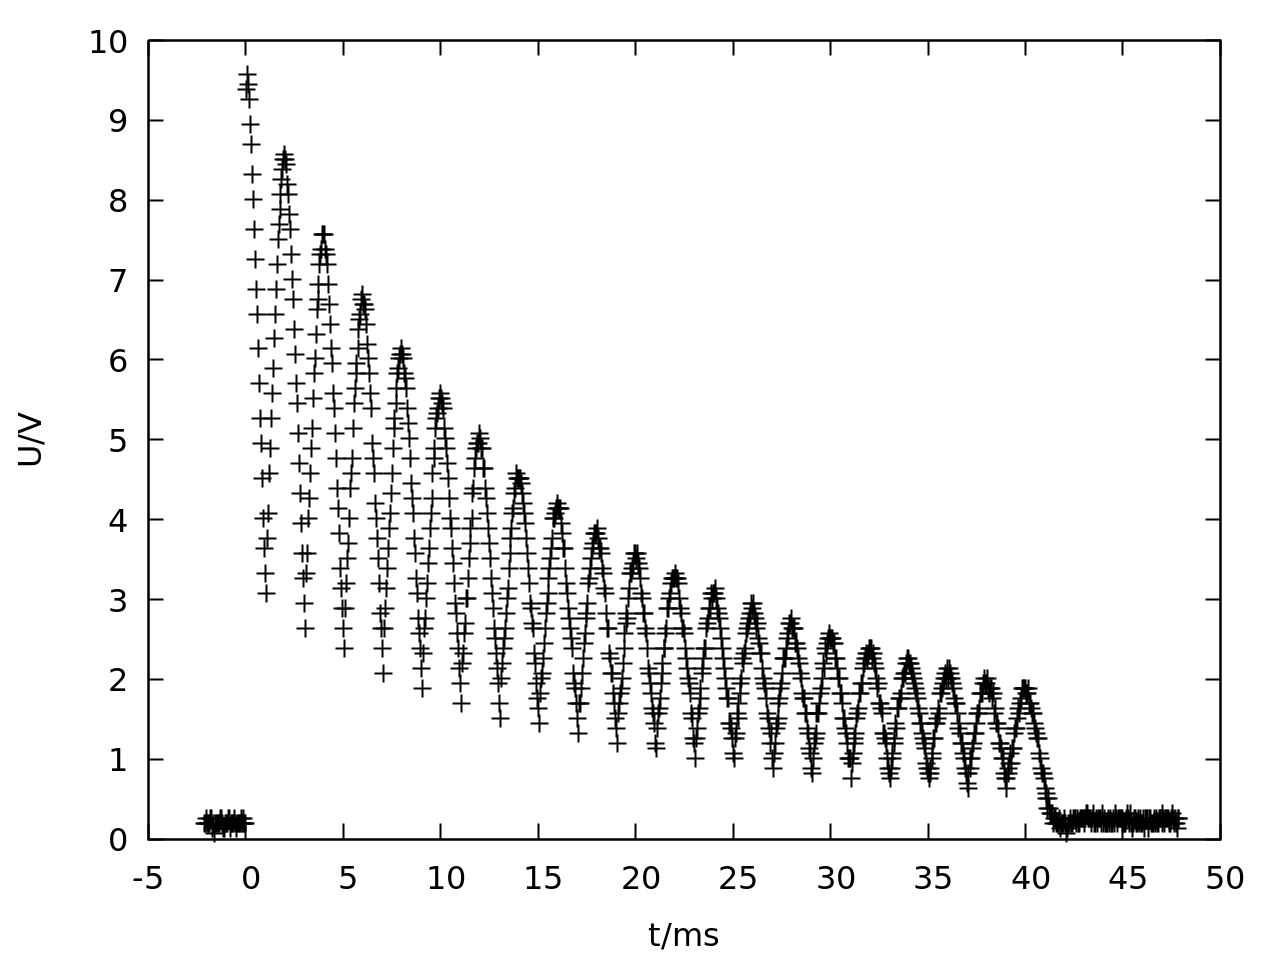
\includegraphics[width=0.75\linewidth]{data/p402_443_data/meiboom_gill_sequenz/plot_161.png}
\caption{(Meiboom-Gill-Sequenz) Nach Änderung der Magnetfeldgradienten}
\label{fig:gill_b}
\end{figure}

Die Ergebnisse der verschiedenen Messungen von $T_2$ sind: $(20,2\pm 0,6) \si{\milli\second},  (19,2\pm 0,3) \si{\milli\second}$ und $(22,4\pm 0,6) \si{\milli\second}$. Die Werte liegen zwar knapp außerhalb der Fehlerbereiche, sie liegen aber trotzdem nah zusammen. Da alle Werte mit unterschiedlichen Methoden gemessen wurden sind auch leichte Unterschiede zu erwarten. Fehlerquellen sind z.B. das Aufsummieren der Fehler in der Carr-Purcell-Sequenz, was eine schnellere Abnahme zur Folge hat (sie hat auch das kleinste gemessene $T_2$).
